\documentclass[conference]{IEEEtran}
\bibliographystyle{IEEEtran}

\usepackage{cite}
\usepackage[latin1]{inputenc}
\usepackage[dvips]{graphicx}
\usepackage{theorem}
\usepackage{algorithmic}
\usepackage{algorithm}
\usepackage{latexsym}
\usepackage{amsmath}

\newlength{\graphwidth}

\newcommand{\fig}[3][scale=0.5]
{
  \vspace{0.3cm}
  \begin{minipage}[t]{0in}
    \vspace{0pt}
    \makebox{\small #2}
  \end{minipage}
  \settowidth{\graphwidth}{\includegraphics[#1]{#3}}
  \nopagebreak\kern-1.5cm
  \begin{minipage}[t]{\graphwidth}
    \vspace{0.2cm} \includegraphics[#1]{#3}
  \end{minipage}
}

\newtheorem{definition}{Definition}

\begin{document}
\title{Implementation of Full Synchronous Composition of
  Discrete Event Models Using IEC 61499 Function Blocks}

\author{\authorblockN{Goran Cengic and Knut �kesson}
\authorblockA{
  Automation Laboratory\\
  Department of Signals and Systems\\
  Chalmers University of Technology\\
  Sweden
}
\and
\authorblockN{Chengyin Yuan and Placid Ferreira}
\authorblockA{
  Department of Mechanical and Industrial Engineering\\
  University of Illinois at Urbana-Champaign\\
  USA
}
}
\maketitle
\begin{abstract}
%   Two methods for the implementation of synchronized
%   execution of the discrete event systems using the IEC
%   61499 function blocks are presented. The first method is
%   suitable for distributed control applications. Each
%   discrete event model is implemented in a single function
%   block type. These models are executed synchronously using
%   a special synchronization function block type. The second
%   method is suitable for non--distributed, i.e. local,
%   control applications and implements all discrete event
%   models that need to be synchronized in one function block
%   type. The methods are presented using a simple
%   manufacturing system. A supervisor for the example has been
%   synthesized using simpler resource models resulting in
%   more efficient synthesis. On the other hand complex models
%   have been used for the execution giving more accurate
%   control.
\end{abstract}


\section{Introduction}
% distributed control systems
In many man--made systems there is a need for distributed
control systems. The need is greatest in cases where the
system is distributed among different geographical locations
or dispersed over large area. Examples of such systems are
manufacturing systems and chemical processing systems.

Developing distributed control systems is costly and error-prone
due to that the existing communication standards are either
vendor dependent or at a low level of abstraction. An
emerging open standard for developing distributed control
system is IEC~61499~\cite{iec:614991:2000},
\cite{rl:mod:2001}. IEC 61499  extends the standard for
Programmable Logic Controller, IEC~61131~\cite{iec:61131},
with functionality for distributed execution of control objects. 

Shorter product life-cycles increases the demands on the
manufacturing system. Since the product, to be produced, in
the manufacturing plant is changing frequently the
production equipment needs to be modified too. The frequent
changes of the system make it time consuming and expensive
to update the control system application to reflect the
changes. The same problem applies to all of the system types
mentioned above and it becomes even larger in mission
critical control applications since the strict requirenment
of guaranteeing the correct operation is imposed. Thus,
there is a need to introduce algorithms and tools to make is
a simple and safe as possible to modify the control system. 

% formal methods and suprevisory control
Many man made systems can, at some abstraction level, be
modeled by discrete event models. A useful class of discrete
event models is the deterministic finite automata. Finite
automata can be used in a formal method,
called suprevisory control theory~\cite{rw:con:1989}, to
automatically generate correct control functions so that the
controlled system exhibits behavior given by some
specification.

% synchronization
In suprevisory control theory the interaction between models
is modeled by synchronization operator. This operator has to
be implemented in control application in order to transfer
theoretical results into operating control system. The
implementation has to be distributable for it to be useful
in control systems for the applications distributed over
geographical area, like those mentioned in the beginning of
the introduction. 

There are existing methods for implementation of
synchronization operator using PLC programming techniques
\cite{hfl:syn:1999,hfl:mod:2001,fh:plc:1998} but the
distribution is hard to achieve in that programming
environment. A new method presented in this paper uses the
emerging standard for distributed control systems to remedy
that.

% paper organisation
Mathematical definitions that are used in the paper are
presented in the next section. After that, the most
important definitions and results of suprevisory control
theory are introduced followed by an exampel showing how
supervisory control theory can be applied in implementation
of control application for a small system. After the example
a method for implementation of the synchronization operator
for any number of synchronized models is presented together
with the argument for the correctness of the implementation.
In Section~\ref{sec:app_SCT} some considerations for
implementation of supervisory control theory in applications
are presented before the conclusion of the paper.



\section{Mathematical Preliminaries}
In~\cite{hmu:int:2003} many important results for automata
are presented. Below, the terminology in this paper is
introduced.\\
\textbf{Definition:} Deterministic Finite Automaton (DFA)\\
A deterministic finite automaton is a 5-tuple defined as
$${A} = \langle Q, \Sigma, \delta, q_i, Q_m\rangle$$
where
$Q$ is a nonempty finite set of \emph{states}, $\Sigma$ is
the \emph{alphabet} which is a finite set of symbols that
denote the occurrence of an event, $\delta:Q\times \Sigma
\rightarrow Q$ is a \emph{transition function}, $q_i \in Q$
is the \emph{initial state} and $Q_m \subseteq Q$ is a set
of \emph{marked states}. $\Box$\\
\textbf{Definition:} Enabled Event Function\\
The enabled event function $\Gamma$ is defined as
$$\Gamma:Q\rightarrow 2^{\Sigma}$$
where $\Gamma(q)$ is the
set of all events $\sigma$ for which $\delta(q,\sigma)$ is
defined. $\Box$\\
Automata are usually visualized by directed graphs with
states represented by nodes, transitions by arrows and
events upon which the transitions occur by labels on the
arrows.

Synchronous composition, \cite{h:com:1985}, is a useful
approach to model the interaction between automata and is
used in this paper to model the interaction between the
system models.\\
\textbf{Definition}: Full Synchronous Composition of two DFAs\\
The full synchronous composition of two DFAs, $A^1$ and
$A^2$, is denoted ${A}^1||{A}^2=\langle
Q,\Sigma,\delta,q_i,Q_m\rangle$ where $Q=Q^1 \times Q^2$,
$\Sigma=\Sigma^1 \cup \Sigma^2$, $q_i=\langle {q^1_{i}},
{q^2_{i}} \rangle$, $Q_m={Q^1_{m}} \times {Q^2_{m}}$ and the
transition function is
\begin{displaymath}
  \begin{array}{l}
    \delta(\langle{q^1,q^2}\rangle,\sigma)=\\
    =\left\{ {\begin{array}{*{10}l}
          {{ \langle \delta ^1 (q^1 ,\sigma ), \delta ^2 (q^2 ,\sigma ) 
              \rangle}} &  \sigma \in \Gamma^1(q^1) \cap \Gamma^2(q^2) \\
          {{ \langle \delta ^1 (q^1 ,\sigma ), q^2 \rangle} } &  \sigma \in 
          \Gamma^1(q^1) \setminus \Sigma^2 \\
          { { \langle q^1, \delta ^2 (q^2 ,\sigma )\rangle}} & \sigma \in 
          \Gamma^2(q^2) \setminus \Sigma^1 \\
          { \rm undefined} & {{\rm otherwise.}}
        \end{array}} \right.
  \end{array}
\end{displaymath} 
where $q^1 \in Q^1$, $q^2 \in Q^2$ and $\sigma \in
\Sigma$. $\Box$
In other words, if an event is in both alphabets and it is
enabled in both automatons, the transitions associated with
it are made simultaneously in both automatons. Otherwise,
only the automaton containing the event in its alphabet
makes the transition. This definition can be extended for
several automata.\\
\textbf{Definition}: Full Synchronous Composition of $n$ DFAs\\
The full synchronous composition of DFAs,
$A^1$, $A^2$ ... $A^n$, is denoted ${A}^1||...||{A}^n=\langle
Q,\Sigma,\delta,q_i,Q_m\rangle$ where 
\begin{eqnarray}
  Q & = & Q^1 \times Q^2 \times ... \times Q^n\nonumber\\
  \Sigma & = & \Sigma^1 \cup \Sigma^2 \cup ... \cup \Sigma^n\nonumber\\
  q_i & = & \langle q^1_i,q^2_i,...,q^n_i \rangle\nonumber\\
  Q_m & = & Q^1_m \times Q^2_m \times ... \times Q^n_m\nonumber
\end{eqnarray}
and the transition function is
\begin{multline}\label{eq:delta}
  \delta(\langle{q^1,...,q^n}\rangle,\sigma)=\\
  =
  \begin{cases}
    {\rm undefined} &, {\rm if\ } \exists A^k:\sigma\in\Sigma^k\land\sigma\notin\Gamma^k(q^k)\\
    \langle q^{1+},\dots,q^{n+}\rangle & {\rm , otherwise}
  \end{cases} 
\end{multline} 
where 
\begin{equation}\label{eq:qi}
  q^{k+}=
  \begin{cases}
    \delta^k(q^k,\sigma) & {\rm if\ }\sigma\in\Gamma^k(q^k)\\
    q^k                  & {\rm if\ }\sigma\notin\Sigma^k
  \end{cases}
\end{equation}
$\Box$\\
What this definiton states is that in a group of automatons
that share one event if there is one automaton that does not
have that event enabled in its current state, than the event
is not allowed to occur in any of the other automatons in
the group. That is, one automaton is able to prevent all the
others from executing an event if it does not enable it at
the same time as all the other automatons. This property of
the definiton is used to construct a supervisor which
prevents events from occurring. The concept of supervisor is
explained further in the next section which introduces the
supervisory control theory.

\section{Supervisory Control Theory}
\label{sec:sct}
Suprevisory control theory provides definitions and results
needed for caluation of allowed behavior of the system from
discrete event models of possible behavior and desired
behavior. The model of the possible behavior is called the
plant, the model of the desired behavior is called the
specification, and the result of the computation is called
the suprevisor.

In the supervisory control theory, the plant is assumed to
generate all events and the purpose of the supervisor is to
prevent the plant from generating events that will violate
the specfication. The assumption that the plant generates
all events might seem like a restriction. However, it is
often possible to introduce a controller between the
supervisor and the resources that initiate the events.
Treating the controller as part of the plant will make the
assumption that all events is generated by the plant a
natural one. In Figure~\ref{fig:sup_plant} such configuration
is shown.
\begin{figure}
  \centering 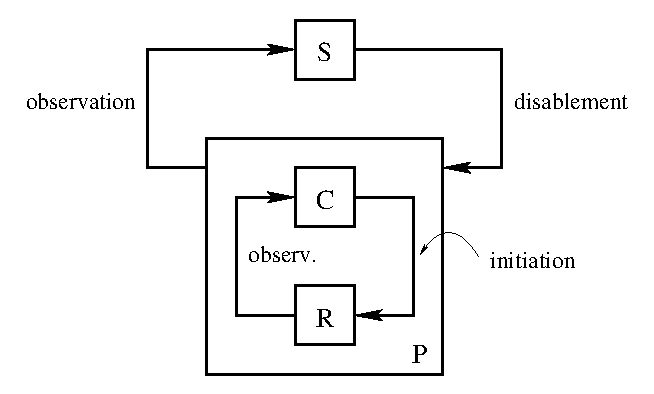
\includegraphics[scale=0.5]{figures/sup_plant}
  \caption{Supervisory control configuration.}
  \label{fig:sup_plant}
\end{figure}

The supervisor $S$ in Figure~\ref{fig:sup_plant} has to
prevent the plant from breaking the specification and from
getting blocked in a state from where it can not reach a
marked state by using as few restrictions of the plant as
possible. By observing the observable events of the plant
and disabling the controlable events of the plant, the
supervisor decides when, and if, it has to limit the
activity of the plant in order to keep the plant's behavior
within the specification. An important result of the
supervisory control theory is that such a supervisor can be
calculated from the models of the plant and specification so
that the system behavior is given by
$$S||P'.$$

In cases when there are several plant models $P_1,..,P_n$
with appropriate specification models $Sp_1,...,Sp_n$ the
supervisor can also be generated and the system behavior
within specification is given by
$$S||P_1||...||P_n.$$
Thus to control the system so that it
satisfies the specification, the synchronous composition of
the plant and supervisor models has to be implemented in the
control software. Using the conventional implementation
methods, i.e. implementing the synchronization using PLC
programming techniques, the solution becomes complex which
makes it difficult, if not impossible, to distribute across
multiple control computers. Next section presents an example
illustrating how the syncrounous composition can be
implemented using the new standard.

\section{Example}
In previous section it is shown that the synchronization
operator is a central concept for the results of supervisory
control theory. Now an example is presented showing how that
theoretical concept can be implemented using IEC 61499
function blocks for a small system before a general method
is given.

Consider a system containing two plants, \texttt{P1} and
\texttt{P2}. The discrete event models for the plants are
shown in the figure~\ref{fig:plants}. All events in the
models are controllable and observable.The desired behavior
of the system is that event \texttt{b} must always precede
event \texttt{c}. The supervisor for this specification can
be generated and is shown in figure~\ref{fig:sup}.
\begin{figure}
  \centering 
  \fig[scale=0.55]{\texttt{P1}}{figures/P1_aut} 
  \fig[scale=0.55]{\texttt{P2}}{figures/P2_aut}
  \caption{Discrete event models of the plants.}
  \label{fig:plants}
\end{figure}
\begin{figure}
  \centering 
  \fig[scale=0.55]{\texttt{S}}{figures/Sp_aut}
  \caption{The model of the supervisor.}
  \label{fig:sup}
\end{figure}
\begin{figure}[!ht]
  \centering 
  \fig[scale=0.5]{\texttt{SYS}}{figures/Sys_aut}
  \caption{The model of possible system behavior while satisfying
    the desired system behavior, $S||P_1||P_2$.}
  \label{fig:sys}
\end{figure}
Full synchronous execution of these models gives the system
that behaves as freely as possible while fulfilling the
specification. The resulting model of the system is shown in
figure~\ref{fig:sys}.

% IEC 61499 intro
The emergin standard IEC 61499 specifies a generic
architecture for measurement and control of industrial
processes. The architecture is based on functional software
units called \textit{function blocks}. The most common type
of function block in an application is basic function block.
It executes algorithms based on the arriving events and
generate new events that are passed on upon the algorithms
execution. The algorithms use the internal variables and the
data associated with the incoming events to update the
internal variables and produce the output data associated
with the outgoing events. What algorithms are invoked is
controlled by the execution control chart (ECC) which is a
automaton with algorithms associated with different states.
The events are boolean expressions involving event inputs,
internal, input, and output variables. In
Figure~\ref{fig:61499_intro} a basic function block type is
shown using the graphical representation.
\begin{figure}
  \centering
  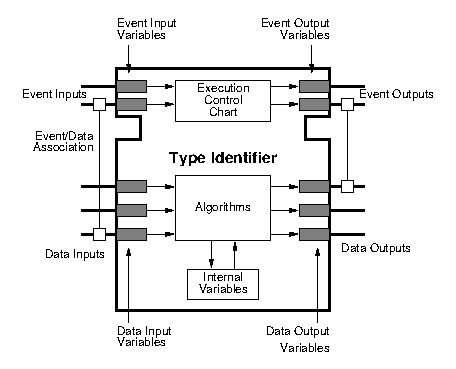
\includegraphics[scale=0.5]{figures/basic_block}\\(a)
  \vskip 5mm
  %\includegraphics[scale=0.5]{figures/basic_ecc}\\(b)
  \caption{(a) The basic function block type and (b) its
    execution control chart.}
  \label{fig:61499_intro}
\end{figure}

The event driven interface enables the distribution of the
function blocks among the multiple control computers.

Function block types that generate the behavior of the plant
and specification models for the example are shown in
figure~\ref{fig:systemFBs}. The event input of each block
type is \texttt{OCCURRED}. It signals that an discrete event
has occurred and that the model should update its state
according to the data inputs. The data inputs are boolean
variables representing the discrete events in the model's
alphabet. For well defined behavior only one of the data
inputs associated with the \texttt{OCCURRED} event must be
\texttt{true} when the event is received. The model's state
is then updated according to the discrete event that this
data input represents and the event output \texttt{DONE} is
generated. It signals that the model has updated its state
and that the data outputs are ready. The data outputs are
boolean variables representing the enabled events after the
model has updated its state, i.e. the events labeling the
transitions that are possible from the new state.

The function block type that is generated according to the
new method presented is shown in figure~\ref{fig:syncFB} and
is called synchronization function block type. The data
inputs and outputs of the block type are application
specific, since they are defined by the models that will be
synchronized. The event input and output, on the other hand,
are the same for all applications which also makes the ECC
of the block type the same for all applications. The ECC for
the block type is shown in figure~\ref{fig:ecc_sync}. The
\texttt{DISABLE\_EVENTS} algorithm associated with the
\texttt{SYNC} state is where the synchronized execution is
implemented. The transition labeled with the ``1'' character
is taken as soon as the \texttt{DISABLE\_EVENTS} algorithm
has finished executing and the \texttt{UPDATE} event is
sent.

\begin{figure}
  \centering
  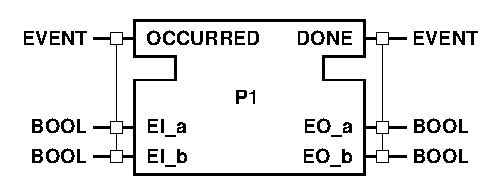
\includegraphics[scale=0.5]{figures/P1}\\(a)
  \vskip 5mm
  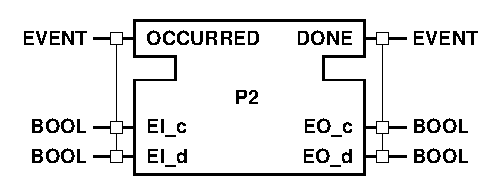
\includegraphics[scale=0.5]{figures/P2}\\(b)
  \vskip 5mm
  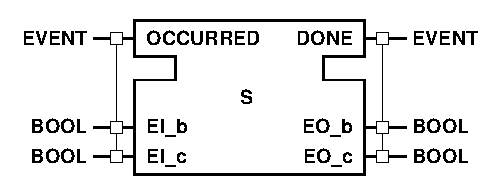
\includegraphics[scale=0.5]{figures/Sp}\\(c)
  \caption{The function block types implementing (a)
    resource 1, (b) resource 2, and (c) specification.}
  \label{fig:systemFBs}
\end{figure}
\begin{figure}
  \centering
  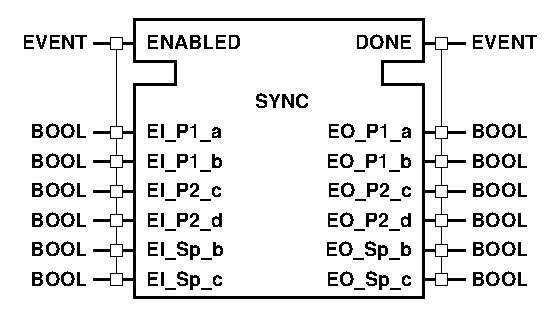
\includegraphics[scale=0.5]{figures/SYNC}
  \caption{The function block type for the synchronization.}
  \label{fig:syncFB}
\end{figure}

The synchronization block reads the enabled events of the
synchronized models and disables the events that are not
enabled in all the models that have that event in their
alphabets. Each boolean data input signals if the event in
the model represented by that input is enabled
(\texttt{true}) or disabled (\texttt{false}). By setting the
corresponding data output to \texttt{false} the
synchronization block signals that the transition labeled by
that event is not allowed to occur in the model during the
next update cycle, if so needed. To calculate each data
output a logical expression consisting of all data inputs
that represent the same event, connected by logical
\texttt{and} operation, is used. This means that if the
event is enabled in all of the models that have the event in
their alphabet it is allowed to occur in the next update
cycle. Otherwise the expression is false and the the event
is disabled. Following implementation of the
\texttt{DISABLE\_EVENTS} algorithm in IEC 61131 structured
text does the computation:

\begin{figure}
  \centering
  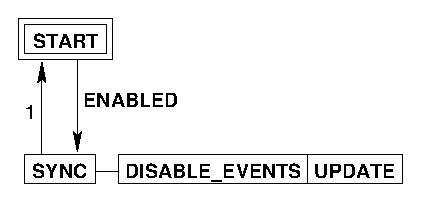
\includegraphics[scale=0.6]{figures/sync_ecc}
  \caption{The execution control chart for the
    synchronization function block type.}
  \label{fig:ecc_sync}
\end{figure}
\begin{figure}
  \centering
  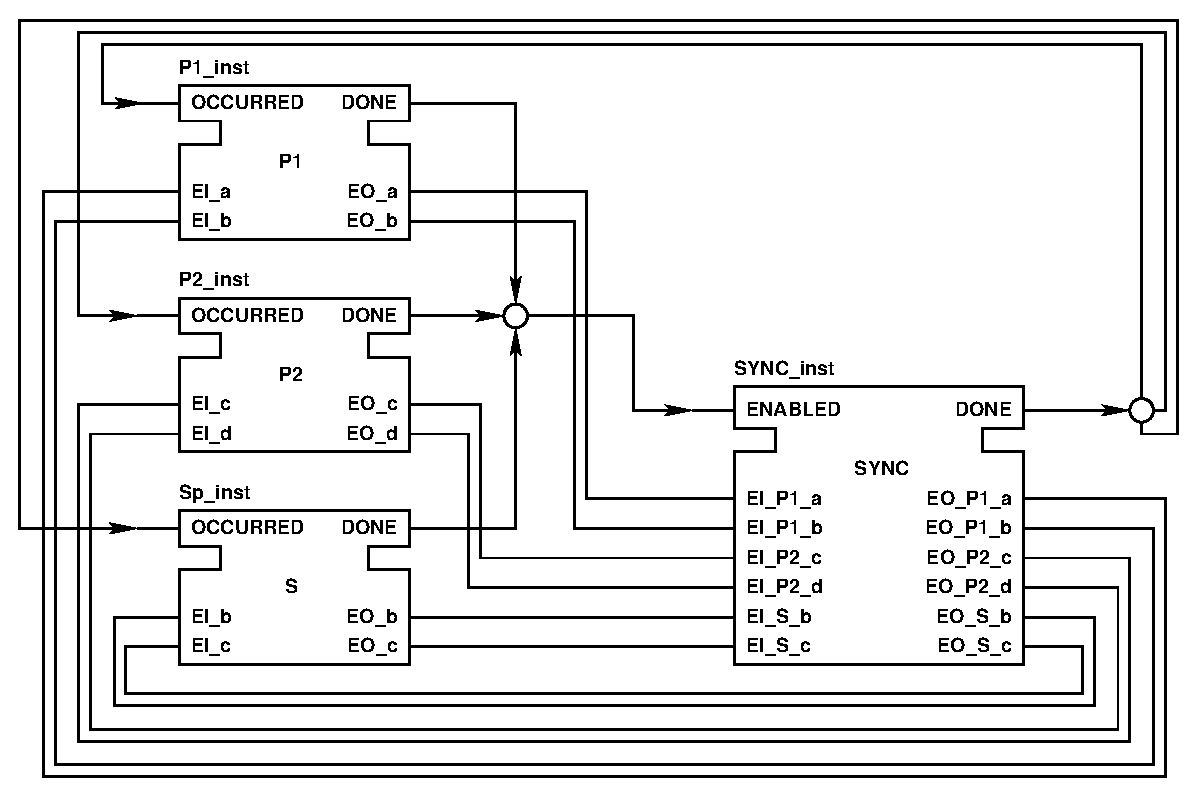
\includegraphics[scale=0.35]{figures/app}
  \caption{The control application for the example.}
  \label{fig:app}
\end{figure}

\begin{verbatim}
EO_R1_a := EI_R1_a;
EO_R1_b := EI_R1_b AND EI_Sp_b;
EO_R2_c := EI_R2_c AND EI_Sp_c;
EO_R2_d := EI_R2_d;
EO_Sp_b := EI_R1_b AND EI_Sp_b;
EO_Sp_c := EI_R2_c AND EI_Sp_c;
\end{verbatim}
Since the event \texttt{a} is in the alphabet of the
\texttt{R1} model only it is always allowed to occur if it
is enabled. The event \texttt{b} is allowed to occur in
\texttt{R1} model only if it is enabled in \texttt{R1} and
\texttt{Sp} models at the same time since it is contained in
both alphabets. The same applies to the event \texttt{b} in
\texttt{Sp} model, hence the same logical expression. Events
\texttt{d} and \texttt{c} are treated in the same manner.


\section{General Method}
The method for implementation of the full synchronous
composition for the general system containing any number of
discrete event models is made up of two major steps. The
first step is creation of the function block types that
generate the behavior of the discrete event models. The
interface that these blocks have to adhere to is shown in
figure~\ref{fig:model_interface}. These blocks are
application specific but they can be automatically generated
from discrete event models~\cite{aff:sup:2003},
\cite{www:sup:2004}.

\begin{figure}
  \centering
  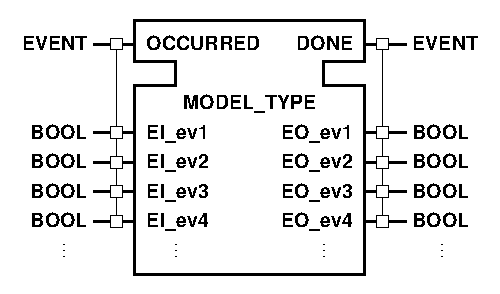
\includegraphics[scale=0.5]{figures/model_interface}
  \caption{The interface definition for the function block
    implementation of the discrete event models.}
  \label{fig:model_interface}
\end{figure}
\begin{figure}
  \centering
  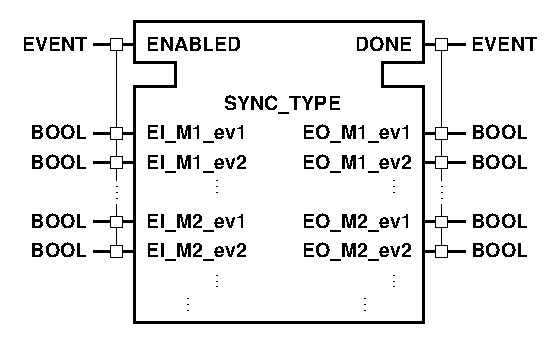
\includegraphics[scale=0.5]{figures/sync_interface}
  \caption{The interface definition for the synchronization
    function block type.}
  \label{fig:sync_interface}
\end{figure}

The second step is creation of the synchronization function
block type. The interface of this block is shown in the
figure~\ref{fig:sync_interface}. The execution control chart
for the function block type is the same as shown in
figure~\ref{fig:ecc_sync} since it is application generic.

The \texttt{DISABLE\_EVENTS} algorithm is also application
specific and it can be generated like this: Let $M$ be the
set of all models for synchronization. For all $m,e$ such
that $m\in M$ and $e\in\Sigma^m$:
\begin{equation}\label{eq:lexp}
  {\rm EO}\_m\_e:=\bigwedge_{\{n:n\in
    M\land e\in\Sigma^n\}}{\rm EI}\_n\_e
\end{equation}
The iteration over all events of all models is for the
generation of the logical expression assignments to all data
outputs, which are represented by EO\_$m$\_$e$. The right
hand side of~(\ref{eq:lexp}) generates the logical expression
that covers all the cases of the synchronization definition.
The first case in~(\ref{eq:delta}) is covered by
$e\in\Sigma^n$ and the data input being \texttt{false} which
gives that EO\_$m$\_$e$ is \texttt{false} and thus the event
is disabled. The first case in equation~\ref{eq:qi} is
covered by $f$ being in the $\Sigma^n\cap\Sigma^m$ and the
data input being \texttt{true}. Finally, the second case in
equation~\ref{eq:qi} is covered by $f$ being in the
$\Sigma^n\cap\Sigma^m$. What is left now is to connect
instances of the model function blocks with the
synchronization function block, which concludes the method.

\section{Application of supervisory control theory}
\label{sec:app_SCT}
Blah blah.

\section{Conclusion}
In many distributed control applications the need for
synchronous execution of discrete event models is present.
The two methods presented in this paper may be used to
implement such synchronous execution by using IEC 61499
function blocks. The first method is useful in case the
function blocks implementing the models that need to be
synchronized have to be distributed across different
computing resources in the control system. It also results
in a slightly more complex function block program. The
second method on the other hand results in a single function
block type but it is only useful when the synchronized
models can fit into single computing resource.

The structure of the function block types in both methods is
obvious. This makes implementation of computer programs for
the generation of such blocks a straight forward task. In
fact, the function block type generation for the second
method is already implemented in the Supremica tool,
\cite{aff:sup:2003} and \cite{www:sup:2004}. Work is under
way to implement automatic generation for the first method
too. Future considerations should be made to accommodate for
the controllable and uncontrollable events in the automatic
generation of the synchronization function block types.

The method and function block programming in general can be
tested using the Function Block Development Kit (FBDK),
\cite{c:fun:2002}. For further information about IEC 61499
function blocks see \cite{c:ope:2002}.

\bibliography{../../../Bibliographies/desbib.bib}

\end{document}

